\documentclass[a0paper,12pt]{article}
\usepackage[landscape,top=5cm,bottom=3cm,right=5cm,left=5cm]{geometry}
\usepackage{graphicx}
\usepackage[T1]{fontenc}
\usepackage{lmodern}
\usepackage{tikz}
\usetikzlibrary{shapes,arrows}
\usepackage{color}
\usepackage{moresize}
\usepackage{lipsum} % dummy text
\usepackage{multicol}

\newenvironment{Figure}
  {\par\medskip\noindent\minipage{\linewidth}}
  {\endminipage\par\medskip}

% This macro creates header.
\newcommand{\HEADING}[1]
{
    \includegraphics[scale=0.25]{./images/heading.png} \vspace{-1cm}
    {\fontsize{2cm}{2em}\selectfont \textcolor{red}{#1}}
    \vspace{2cm}
}


\tikzset{
  every overlay node/.style={
    draw=black,fill=white,rounded corners,anchor=north west,
  },
}
% Usage:
% \tikzoverlay at (-1cm,-5cm) {content};
% or
% \tikzoverlay[text width=5cm] at (-1cm,-5cm) {content};
\def\tikzoverlay{%
   \tikz[baseline,overlay]\node[draw=white,every overlay node]
}%

\begin{document}

\begin{tikzpicture}[remember picture,overlay] 
    \node[opacity=1.0] (background) at (current page.center) {
    
\includegraphics[width=\paperwidth,height=\paperheight]{./background.jpg}
};
\end{tikzpicture}


\begin{minipage}{\textwidth}
    \centering
    \fontsize{4cm}{1em}\selectfont \textcolor{red}{Modelling Memory Across Scale}
    \\
    \fontsize{1.5cm}{1em}\selectfont Aditya Gilra, Aviral Goel, Dilawar Singh,
    Harsha Rani, Sahil Moza, Subhasis Ray, Upinder Bhalla
\end{minipage}



%% Three columns
\vspace{5cm}
\setlength{\columnsep}{6cm}
\begin{multicols}{3}
    
%%%%%%%%%%%% Column 1
\begin{Figure}

    \HEADING{Introduction}

    \begin{Figure}
     {\HUGE Memory and plasticity involve brain mechanisms from molecular scale
         to enormous networks. \\};

     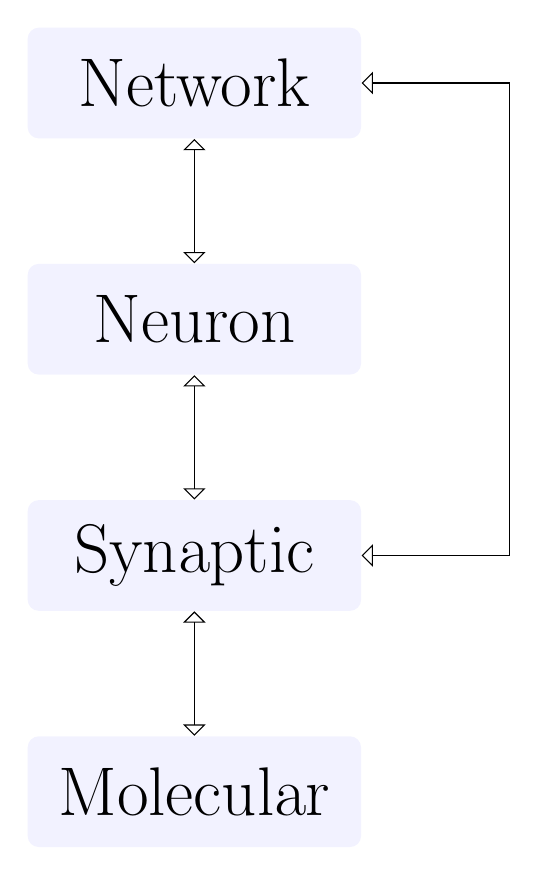
\begin{tikzpicture}[
        block/.style={
             rectangle
            , align=center
            , fill=blue!5
            , rounded corners
            , text width=4cm
            , node distance=3cm
            , font=\fontsize{1cm}{1em}\selectfont
            , minimum height=4em
        }
        ]
        \node[block] (network) {Network};
        \node[block,below of=network] (neuron)  {Neuron};
        \node[block,below of=neuron] (synaptic) {Synaptic};
        \node[block,below of=synaptic] (molecular) {Molecular};

        \draw[block,open triangle 90-open triangle 90] (molecular) -- (synaptic);
        \draw[block,open triangle 90-open triangle 90] (neuron) -- (synaptic);
        \draw[block,open triangle 90-open triangle 90] (network) -- (neuron);

        \draw[open triangle 90-open triangle 90] (network) -- ++(4,0) --
        ++(0,-5) |- (synaptic);
        ;

    \end{tikzpicture} 
     \begin{tikzpicture}
         \centering
         \node [] (image) at (0,-1) {
             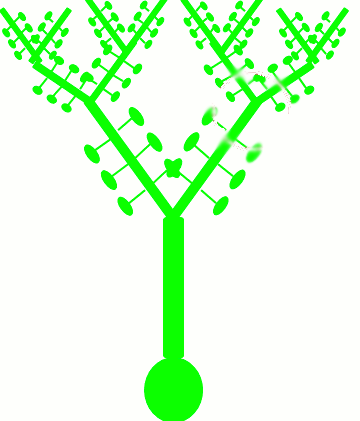
\includegraphics[scale=0.3,angle=-30]{./images/single_cell.png}
         };

         \foreach \i in {-3,...,3}
         \foreach \j in {-3,...,3}
         {
             \node[fill=yellow!30,thin,circle] (n\i\j) at (\i, \j) {};
         }
         \node[below=4cm] {\LARGE A neuron embed in network};
     \end{tikzpicture} 
    \begin{tikzpicture}
        \node[] (image) {
            \includegraphics[width=0.5\textwidth]{./images/Gallery_Moose_Multiscale.png}
        };
    \end{tikzpicture} %
    \end{Figure}

    \HEADING{Multiscale Modeling in MOOSE}

    \begin{Figure}

        {\HUGE We have developed \textcolor{red}{MOOSE}, the Multiscale Object
            Oriented Simulation Environment, to model plasticity across scales.}

        {\HUGE \textbf{Some projects using MOOSE}}
        
        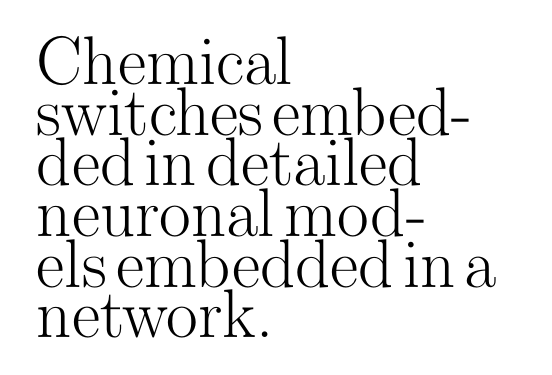
\begin{tikzpicture}

            \node[below=6cm, text width=0.5\textwidth] {\Huge
                Chemical switches embedded in detailed neuronal models embedded in a
                network.
            };

        \end{tikzpicture} %
        \begin{tikzpicture}

            \node[] (image) {
                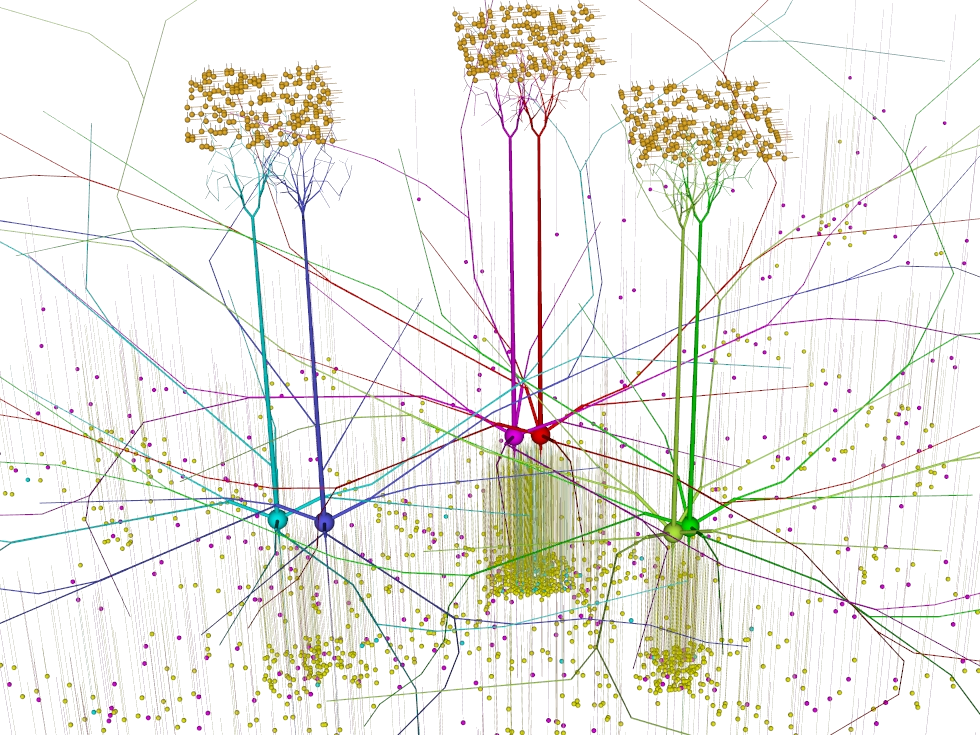
\includegraphics[width=0.5\textwidth]{./images/fullmodel_moogli.png}
            };

            \node[below=6cm,text width=0.5\textwidth]{ \Huge
                Network coding and computation in olfaction and sematosensory
                cortex.
            };

        \end{tikzpicture}%

        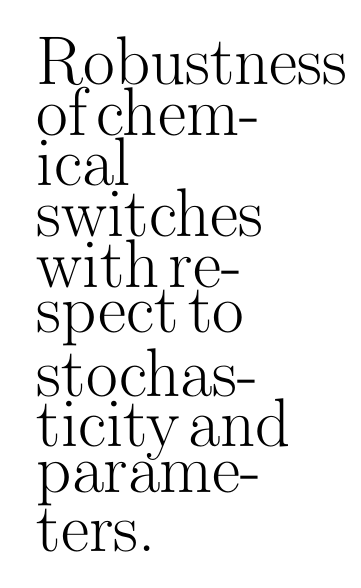
\begin{tikzpicture}
            \node[text width=0.3\textwidth] {\Huge
                Robustness of chemical switches with respect to stochasticity and
                parameters.
            };

        \end{tikzpicture}

    \end{Figure}

\end{Figure}

%% Column 2

\begin{Figure}
    \HUGE
    Content of column 2.
\end{Figure}

%% Column 3
\begin{Figure}
    
    \HEADING{Summary}

    \HUGE We use models to
    \begin{itemize}
            
        \item Integrate many scales of neuronal data with basic
            physical/chemical principles.
        \item Explain phenomenon of plasticity, activity and neuronal coding.
        \item Predict circuit mechanisms, plasticity rules, and emergent
            phenomena such as \emph{decorrelation}, \emph{robustness}, and
            \emph{memory decay}.

    \end{itemize}

    \textbf{We have developed MOOSE to carry out these simulations}.

\end{Figure}

\end{multicols}

\end{document}
